\documentclass[pdf]{beamer}

\title{\textbf{Bayesian A/B testing with Python}}
\author{Bogdan Kulynych}

%% Theme
%\usetheme{boxes}
%\usecolortheme{seahorse}
\setbeamercovered{transparent=20}

\usepackage{amsmath}
\usepackage{parskip,graphics,tikz}
\usepackage{pgfplots}
\usetikzlibrary{arrows,positioning,shapes}

\usepackage{listings,textcomp,color}

\definecolor{mygreen}{rgb}{0,0.6,0}
\definecolor{mygray}{rgb}{0.5,0.5,0.5}
\definecolor{mymauve}{rgb}{0.58,0,0.82}

\lstset{
  language=python,
  backgroundcolor=\color{white},   % choose the background color
  basicstyle=\ttfamily\footnotesize,  % size of fonts used for the code
  breaklines=true,                 % automatic line breaking only at whitespace
  captionpos=b,                    % sets the caption-position to bottom
  commentstyle=\color{mygreen},    % comment style
  escapeinside={\%*}{*)},          % if you want to add LaTeX within your code
  keywordstyle=\color{blue},       % keyword style
  stringstyle=\color{mymauve},     % string literal style
  frame=single,tabsize=2
}

\tikzset{
  a/.style={draw,thick,rounded corners,fill=blue!20,inner sep=.3cm},
  b/.style={draw,thick,rounded corners,fill=red!20,inner sep=.3cm},
}


\begin{document}

\pgfmathdeclarefunction{gauss}{2}{%
  \pgfmathparse{1/(#2*sqrt(2*pi))*exp(-((x-#1)^2)/(2*#2^2))}%
}


\frame{\titlepage}


\section{A/B testing}


\begin{frame}{A/B testing}
	
	Behavioral research study designed to answer specific questions about behavioral interventions. Theoretical developments come from clinical trials. 
	
	We focus on Web development:
	
	\begin{itemize}
		\item Small set of (web page) variations: $A, B, C, \dots$
		\item Metrics to compare variations: profit gained, time spent on the page,  signup rate
		\item Use of statistical methods to estimate the metrics
	\end{itemize}
		
	To be contrasted to \emph{personalization}.
	
\end{frame}


\section{Classical approach} 


\begin{frame}{Classical approach}

Suppose there are two variations of Web page design: $A$ and $B$.

\vspace{.5cm}

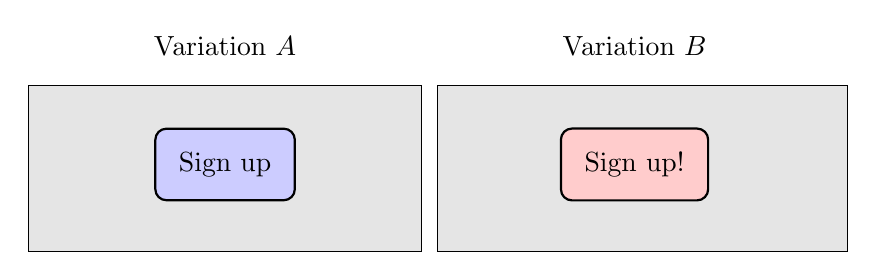
\begin{tikzpicture}
	
	\draw[fill=gray!20] (-1.7cm,-1.1cm) rectangle (3.3cm,1cm) {};
	\node[a] at (.8cm,0cm) (a) {Sign up};
	\node at (.8cm,1.5cm) {Variation $A$};
	
	\draw[fill=gray!20] (8.7cm,-1.1cm) rectangle (3.5cm,1cm) {};
	\node[b] at (6cm,0cm) (b) {Sign up!};
	\node at (6cm,1.5cm) {Variation $B$};

\end{tikzpicture}

\vspace{.5cm}

\begin{itemize}
	\item We want to find out which one will probably produce more signups
	\item Randomly show visitors one of the variations and log the results
\end{itemize}

\end{frame}


\begin{frame}{Classical approach}{Model}

\begin{itemize}
	\item Let $A, B$ be finite binary populations $ A^{(i)}, B^{(i)}.$ $a^{(i)}, b^{(i)} \in \{0, 1\}$.

	\item Fix true signup rates $p_A, p_B$: 
	$$ A \sim \text{Bernoulli}(p_A),\ B \sim \text{Bernoulli}(p_B) $$

	\item Assume that by logging views and signups we obtain random samples of the populations $X_A, X_B$:
	$$x_A^{(i)} \sim \text{Bernoulli}(p_A),\ x_B^{(i)} \sim \text{Bernoulli}(p_B) \text{ are i.i.d RVs} $$
	\item We want to estimate the difference between true population parameters $p_A, p_B$. They are \emph{fixed but unknown}.
\end{itemize}

\end{frame}


\begin{frame}{Classical approach}{Hypothesis testing}
Two sample $t$-test is often used:
$$ H_0: p_A = p_B,\quad H_1: p_A > p_B,\quad H_2: p_A < p_B $$
Compute $T$-statistic:
$$ T = \frac{\bar X_A - \bar X_B}{\sigma_{\hat p_A - \hat p_B}}$$
where $\hat p_A = \bar X_A,\ \hat p_B = \bar X_B$ are sample average values, and
$$\sigma_{\hat p_A - \hat p_B}^2 = \frac{\sigma_{X_A}^2}{n_{X_A}} + \frac{\sigma_{X_B}^2}{n_{X_B}}$$
\end{frame}


\begin{frame}{Classical approach}{Hypothesis testing}
Under $H_0: p_A = p_B$ $T$-statistic is t-distributed for small sample sizes, and standard normal distributed if sample sizes are big enough. 

$P(X~|~H_0)$ can be found then. Example for $\alpha=0.95$ and standard normal distribution:

\begin{tikzpicture}
\begin{axis}[
  no markers, domain=-5:5, samples=100,
  axis lines*=left,
  every axis y label/.style={at=(current axis.above origin),anchor=south},
  every axis x label/.style={at=(current axis.right of origin),anchor=west},
  height=4cm, width=12cm,
  xtick={-1.96,1.96}, ytick=\empty,
  enlargelimits=false, clip=false, axis on top,
  grid = major
  ]

  \addplot [very thick,cyan!50!black] {gauss(0, 1)};

\draw [yshift=-0.8cm, latex-latex](axis cs:-5,0) -- node [fill=white] {$p_A < p_B$} (axis cs:-1.96,0);
\draw [yshift=-0.8cm, latex-latex](axis cs:-1.96,0) -- node [fill=white] {$p_A = p_B$} (axis cs:1.96,0);
\draw [yshift=-0.8cm, latex-latex](axis cs:1.96,0) -- node [fill=white] {$p_A > p_B$} (axis cs:5,0);
\end{axis}

\end{tikzpicture}

\end{frame}


\section{Bayesian vs. frequentist approach }


\begin{frame}{Classical approach}{Problems}

\begin{itemize}
	\item Easy to misuse: $\alpha$ controls only type I errors, type II are often forgotten. For every parameter value, there's a certain sample size that needs to be obtained before drawing any conclusions.
	\item Reliance on large numbers: LLN and CLT.
	\item Reasoning based on $\text{P}(\text{data}~ | ~\text{hypothesis})$ and finite amount of hypotheses about the fixed parameters. $\text{P}(\text{parameters}~ | ~\text{data})$ is arguably more appropriate and more general, but doesn't make sense within the given model (\emph{parameters are fixed}).
	\item Confidence intervals like $I: P(\text{parameter} \in I ~|~\text{data}) = \gamma $ often misinterpreted: it generally does not mean that \emph{probability of parameter being in the interval $I$ is $\gamma$}, since parameters are fixed.
\end{itemize}

\end{frame}


\begin{frame}{Bayesian approach}{Model}

	\begin{itemize}
		\item \emph{Let true signup rates $p_A, p_B$ be independent random variables}. Let \emph{prior} distributions of $p_A$ and $p_B$ be Beta-distributed:
		$$ p_A \sim \text{Beta}(\alpha_A, \beta_A),\ p_B \sim \text{Beta}(\alpha_B, \alpha_B) $$
												
		\item Assume that the likelihood of data obtained by logging views and signups is binomial. Let number of signups $k_A = |\{x_A^{(i)}=1\}|$, number of views $n_B = |X_A|$:
		$$ \text{P}(X_A ~|~ p_A) = \text{Binomial}(k_A; n_A, p_A).  $$
		Analogically, for $p_B$.
		\item We want to find $P(p_A > p_B ~|~X)$, $P(p_A < p_B ~|~ X)$ and \emph{lifts} $\frac{p_B - p_A}{p_A}$ and $\frac{p_A - p_B}{p_B}$.
	\end{itemize}

\end{frame}


\begin{frame}{Bayesian approach}{Bayes theorem}
	\begin{eqnarray*}
	\text{P}(p_A ~|~ X_A) &=& \frac{\text{P}(X_A ~|~ p_A) \cdot \text{P}(p_A)}{\text{P}(X_A)} \propto \text{P}(X_A ~|~ p_A) \cdot \text{P}(p_A) \\
	&=& {n_A\choose k_A} p_A^{k_A} (1-p)^{n_A - k_A}\ \frac{1}{B(\alpha_A, \beta_A) p_A^{1-\alpha_A} (1-p_A)^{1-\beta_A}} \\
	&=& \text{Beta}(\alpha_A + k_A, \beta_A + n_A - k_A)
	\end{eqnarray*}
	
	$\text{P}(p_A ~|~ X_A)$ is called \emph{posterior} distribution. We can trivially compute point estimates $\text{E}[p_A~|~X_A]$, \emph{credible intervals} $I: \text{P}(p_A \in I~ | ~X_A) = \gamma$. 
	
	Using Monte Carlo methods, we can compute $P(p_A < p_B ~|~ X)$ and lifts.
	
\end{frame}


\begin{frame}{Bayesian approach}{Summary}

	\begin{itemize}
		\item Similar assumptions (independent Bernoulli trials, implied by Binomial likelihood)
		\item No reliance on big numbers (in theory)
		\item Instead of finding $\text{P}(\text{data} ~|~ \text{hypothesis})$ for a set of predefined hypotheses about the parameters, we integrate over all possible values of parameters and get $\text{P}(\text{parameter} ~| ~\text{data})$. This is more general approach than hypothesis testing.
		\item We can find \emph{credible intervals} which are easy to interpret right.
		\item Using Monte Carlo techniques, we can calculate any function of the parameters we want (like lift), and assume any likelihoods we want (at the cost of computation)
	\end{itemize}
\end{frame}


\begin{frame}[fragile]{Bayesian approach}{Code}

	We can implement Bayesian A/B testing using \emph{numpy} and \emph{scipy}, and optionally \emph{PyMC} for Monte Carlo methods.
	
	\begin{lstlisting}
import numpy as np
from scipy import stats

data = {
	'A': { 'views': 42, 'signups': 2 },
	'B': { 'views': 85, 'signups': 11 }
}

posteriors = { variation: stats.beta(logs['signups'], logs['views'] - logs['signups'])
      for variation, logs in data.items() }

	\end{lstlisting}
	
\end{frame}


\begin{frame}[fragile]{Bayesian approach}{Code (cont.)}
	
	\begin{itemize}
	\item Point estimates:
	
	\begin{lstlisting}
		print(posteriors['A'].mean())
	\end{lstlisting}
	
	$ \text{E}[p_A~|~X] = 5.81\%,\ \text{E}[p_B~|~X] = 13.37\% $.
	
	\vspace{.5cm}
	
	\item 95\%-Credible intervals
	
	\begin{lstlisting}
		print(posteriors['A'].ppf(0.025), posteriors['A'].ppf(0.975))
	\end{lstlisting}
	
	$ \text{P}(1.00\% < p_A < 14.41\%) = 0.95 $, $\text{P}(7.07\% < p_B < 21.28\%) = 0.95 $
	
	\end{itemize}
	
\end{frame}


\begin{frame}[fragile]{Bayesian approach}{Code (cont.)}

	\begin{itemize}
		\item Monte Carlo approach to compute $P(p_B > p_A~|~X) \approx \frac{1}{n}\sum_i \mathbb{I}[y_A^{i} > y_B^{i}]$ and expected lift:
					
		\begin{lstlisting}
			size = 10000
			samples = { variation: posterior.sample(size) for variation, posterior in posteriors.items() }
			
			dominance = np.mean(samples['B'] > samples['A'])
			lift = np.mean((samples['B'] - samples['A']) / samples['A'])
		\end{lstlisting}
		
		Variation B performs better, so $P(p_B > p_A) = 92.90\%$. Expected lift of signup rate under variation B is $271.68\%$
		
	\end{itemize}

\end{frame}


\begin{frame}[fragile]{Bayesian approach}{\emph{trials} library}

I wrote a small library for running Bayesian A/B testing called \emph{trials} that can do all of the above.

\begin{lstlisting}
from trials import Trials

test = Trials(['A', 'B'], vtype='bernoulli')

test.update({
    'A': (2, 40),
    'B': (11, 79),
})
\end{lstlisting}
\end{frame}


\begin{frame}[fragile]{Bayesian approach}{\emph{trials} library | statistics}

\begin{itemize}
	\item $\text{P}(p_A > p_B ~|~ X)$:
\begin{lstlisting}
dominances = test.evaluate('dominance')
\end{lstlisting}

	\item Expected lift $\text{E}(\frac{p_B - p_A}{p_A} ~|~ X)$:
\begin{lstlisting}
lifts = test.evaluate('expected lift')
\end{lstlisting}

	\item Lift 95\%-credible interval:
\begin{lstlisting}
intervals = test.evaluate('lift CI', level=95)
\end{lstlisting}
\end{itemize}

Available statistics for Bernoulli experiments: expected posterior, posterior CI, expected lift, lift CI, empirical lift, dominance

\end{frame}


\begin{frame}{Bayesian approach}{\emph{trials} library}

Get it on \texttt{github.com/bogdan-kulynych/trials}.

Suggestions and corrections welcome.

\end{frame}


\end{document}
